\chapter{Algoritmos Divide y Vencerás}\label{dyv}

\section{Enunciado}\label{dyv-enunciado}

Dado un árbol de búsqueda almacenado en preorden, se desea añadir un algoritmo eficiente que reconstruya el árbol mediante su matriz de adyacencia.
Por ejemplo, para el siguiente vector:

\[\Big(7, 4, 3, 6, 5, 8, 10\Big)\]

La salida sería la matriz:

\[
\begin{array}{c||c|c|c|c|c|c|c|c|c|c|c}
& \text{\small{1}} & \text{\small{2}} & \text{\small{3}} & \text{\small{4}} & \text{\small{5}} & \text{\small{6}} & \text{\small{7}} & \text{\small{8}} & \text{\small{9}} & \text{\small{10}} \\
\hline
\hline
\text{\small{1}}  & 0 & 0 & 0 & 0 & 0 & 0 & 0 & 0 & 0 & 0 \\
\hline
\text{\small{2}}  & 0 & 0 & 0 & 0 & 0 & 0 & 0 & 0 & 0 & 0 \\
\hline
\text{\small{3}}  & 0 & 0 & 0 & 0 & 0 & 0 & 0 & 0 & 0 & 0 \\
\hline
\text{\small{4}}  & 0 & 0 & 1 & 0 & 0 & 1 & 0 & 0 & 0 & 0 \\
\hline
\text{\small{5}}  & 0 & 0 & 0 & 0 & 0 & 0 & 0 & 0 & 0 & 0 \\
\hline
\text{\small{6}}  & 0 & 0 & 0 & 0 & 1 & 0 & 0 & 0 & 0 & 0 \\
\hline
\text{\small{7}}  & 0 & 0 & 0 & 1 & 0 & 0 & 0 & 1 & 0 & 0 \\
\hline
\text{\small{8}}  & 0 & 0 & 0 & 0 & 0 & 0 & 0 & 0 & 0 & 1 \\
\hline
\text{\small{9}}  & 0 & 0 & 0 & 0 & 0 & 0 & 0 & 0 & 0 & 0 \\
\hline
\text{\small{10}} & 0 & 0 & 0 & 0 & 0 & 0 & 0 & 0 & 0 & 0 \\
\hline
\end{array}
\]

Que representa el árbol:

\begin{center}
\begin{tikzpicture}[grow'=down]
\Tree
	[.$7$
		[.$8$
			$10$
			\edge[blank]; $\ $
		]
		[.$4$
			[.$6$
				\edge[blank]; $\ $
				$5$
			]
			$3$
		]
	]
\end{tikzpicture}
\end{center}

\section{Algoritmo básico}\label{dyv-basico}

Sabemos que un árbol binario de búsqueda está ordenado de forma que, para cada subárbol, el nodo hijo izquierdo es menor que el padre y el nodo hijo derecho es mayor que el padre pero menor que el resto de ancestros.
De esta forma, podemos recuperarlo únicamente conociendo su estructura en preorden.

Un algoritmo básico de reconstrucción del árbol mediante la matriz de adyacencia debería iterar por los elementos en preorden del árbol e ir comprobando su posición en base a los elementos anteriores.
Planteamos las siguientes preguntas para su desarrollo:

\pagebreak

\begin{itemize}
	\item ¿El nodo examinado es un hijo del anterior?
	\begin{itemize}
		\item Si es un hijo, ¿lo es a la izquierda o a la derecha?
		\item Si no es lo es, ¿de qué nodo es hijo?
	\end{itemize}
	\item ¿Hasta dónde debemos retroceder en el preorden para encontrar el padre?
\end{itemize}

Dado a que estamos trabajando en preorden, se nos garantiza que un nodo de valor inferior al anterior es hijo izquierda de éste.
Si es hijo a la derecha o no es hijo, podemos recorrer el vector en preorden en orden inverso hasta encontrar el valor más alto, que se garantiza que será el padre del nodo al estar trabajando en preorden.
Por tanto, tenemos el siguiente algoritmo expresado en pesudocódigo:

\begin{lstlisting}[language=Python]
for i in raiz..tope-1 do
	if preorden[i+1] < preorden[i]
		# Identificar nodo i como el padre del nodo i+i
	else for j in reverse(i..raiz+1)
		mas_alto = 0 # Valor más alto encontrado

		if pre[j] > mas_alto
			mas_alto = pre[j];

		# Identificar nodo de valor más alto encontrado como el padre del nodo i+i
\end{lstlisting}

Podemos implementarlo en C++ aceptando cuatro argumentos:

\begin{itemize}
	\item\texttt{unsigned* pre}\textbf{:} El vector en preorden.
	\item\texttt{unsigned raiz}\textbf{:} La posición de inicio del vector en preorden.
	\item\texttt{unsigned tope}\textbf{:} La posición siguiente al fin del vector en preorden.
	\item\texttt{bool** matriz}\textbf{:} La matriz de adyacencia a rellenar.
\end{itemize}

\begin{lstlisting}[language=C++]
void Sencillo (unsigned* pre, unsigned raiz, unsigned tope, bool** matriz) {
	for (unsigned i=raiz; i<tope; i++) {
		if (i+1 < tope && pre[i+1]<pre[i]) {
			matriz[pre[i]-1][pre[i+1]-1] = true;
		}
		else if (i+1 < tope) {
			unsigned mas_alto = 0;

			for (unsigned j=i; j>raiz; j--) {
				if (pre[j] > mas_alto)
					mas_alto = pre[j];
			}

			matriz[mas_alto-1][pre[i+1]-1] = true;
		}
	}
}
\end{lstlisting}

\section{Resolubilidad por \textit{DyV}}\label{dyv-resolubilidad}

Para poder resolver un problema mediante un algoritmo Divide y Vencerás el caso inicial debe poder ser divisible en subcasos pequeños cuyas soluciones puedan ser combinadas para obtener la solución del caso inicial.
También debemos tener un caso base indivisible o un algoritmo básico que resuelva el problema.

Como demostramos en \S\ref{dyv-basico}, tenemos un algoritmo básico que resuelve el problema, por lo que podemos considerar cumplida esta condición.
Dado que estamos trabajando con un árbol, la división del problema en casos más pequeños es inherente al mismo, ya que su estructura es, por definición, recursiva.
Cada nodo del árbol binario de búsqueda tiene, como máximo, dos nodos hijos que podemos considerar raíces de los subárboles que forman con todos sus nodos descendientes.

\begin{center}
\begin{tikzpicture}[grow'=down]
\Tree
	[.$7$
		[.$8$
			$10$
			\edge[blank]; $\ $
		]
		[.$4$
			[.$6$
				\edge[blank]; $\ $
				$5$
			]
			$3$
		]
	]
\end{tikzpicture}
$\ \ \ \ \ \ \ \ \ \ $
\begin{tikzpicture}[grow'=down]
\Tree
	[.$4$
		[.$6$
			\edge[blank]; $\ $
			$5$
		]
		$3$
	]
\end{tikzpicture}
$\ \ \ \ \ \ \ \ \ \ $
\begin{tikzpicture}[grow'=down]
\Tree
	[.$8$
		$10$
		\edge[blank]; $\ $
	]
\end{tikzpicture}
\end{center}

También identificamos como caso base los nodos hoja, que son indivisibles por no  tener nodos descendientes.

\section{Algoritmo \textit{DyV}}\label{dyv-dyv}

Para resolver este problema mediante un algoritmo Divide y Vencerás tenemos en cuenta la estructura recursiva inherente a los árboles, en los que cada nodo y sus hijos son subárboles del árbol formado por su padre.
Conociendo las propiedades del árbol binario de búsqueda detalladas en \S\ref{dyv-basico} sabemos que, dado un vector que representa un árbol binario de búsqueda en preorden, podemos dividirlo en su raíz, el primer elemento; el subárbol derecho, formado por el primer elemento de valor superior a la raíz y todos los restantes hasta el final del árbol; y el subárbol izquierdo, formado por todos los elementos desde el siguiente a la raíz hasta el primer elemento del subárbol derecho.

\[
\Big(7, 4, 3, 6, 5, 8, 10\Big) \longrightarrow
\begin{cases}
	7          & \text{Raíz} \\
	8, 10      & \text{Subárbol derecho} \\
	4, 3, 6, 5 & \text{Subárbol izquierdo} \\
\end{cases}
\]

De esta forma, vamos dividiendo el árbol en subárboles menores mientras vamos identificando los hijos de las raíces de los subárboles hasta llegar a las hojas.

\begin{lstlisting}[language=Python]
i=raiz # Buscador de la raíz del subárbol derecho

do i=i+1 until preorden[i]>preorden[raiz]

if i < tam_preorden
	# Identificar nodo i como hijo derecho del nodo raíz
	# Identificar nodo raíz-1 como hijo izquierdo del nodo raíz
	Recursion(subarbol_izquierdo)
	Recursion(subarbol_derecho)
else if preorden[raiz] != preorden[i-1]
	# Identificar nodo i como hijo derecho del nodo raíz
	Recursion(subarbol_izquierdo)
\end{lstlisting}

Podemos implementarlo en C++ aceptando los mismos cuatro argumentos que la implementación de \S\ref{dyv-basico}:

\begin{lstlisting}[language=C++]
void DyV (unsigned* pre, unsigned raiz, unsigned tope, bool** matriz) {
	unsigned i;

	for (i=raiz+1; i<tope && pre[i]<pre[raiz]; i++);

	if (i<tope) {
		matriz[pre[raiz]-1][pre[raiz+1]-1] = true;
		matriz[pre[raiz]-1][pre[i]-1] = true;
		DyV (pre, i, tope, matriz);
		DyV (pre, raiz+1, i, matriz);
	}
	else if (pre[raiz] != pre[i-1]) {
		matriz[pre[raiz]-1][pre[i-1]-1] = true;
		DyV (pre, raiz+1, i, matriz);
	}
}
\end{lstlisting}

\section{Estudio de la eficiencia}\label{dyv-eficiencia}

\subsection{Algoritmo básico}\label{dyv-eficiencia-basico}

Este primer algoritmo contiene un bucle \texttt{for} externo con inicialización, comprobación y actualización de eficiencia constante, que se ejecuta de $tope-raiz$ veces, por lo que su eficiencia es $O(n)$.
En su interior tenemos un bloque \texttt{if}, cuya comprobación y cuerpo se ejecutan todas en tiempo constante, por lo que su eficiencia total es $O(1)$.
Contra este bloque \texttt{if} tenemos un bloque \texttt{else if} de comprobación en tiempo constante que contiene un bucle \texttt{for}.
Este segundo bucle cuenta con inicialización, comprobación actualización y cuerpo constantes y que se ejecuta $i-raiz$ veces, siendo su eficiencia $O(n)$.

Por tanto, por la regla del producto, \textbf{el algoritmo tiene una eficiencia de} $\boldsymbol{O(n^2)}$.

\subsection{Algoritmo \textit{DyV}}\label{dyv-eficiencia-dyv}

Para este algoritmo contamos con un bucle \texttt{for} sin cuerpo y con inicialización, comprobación y actualización de eficiencia constante que se ejecuta como máximo $tope-raiz$ veces, de forma que su eficiencia es $O(n)$.
Tras este bucle, encontramos un bloque \texttt{if} de comprobación constante y cuerpo con dos llamadas recursivas y resto constante y un bloque \texttt{else if} de iguales características que el bloque \texttt{if} pero con una sola llamada recursiva, por lo que tomamos el bloque \texttt{if} para analizar la eficiencia.

Como describimos en \S\ref{dyv-dyv}, este algoritmo divide el árbol en subárboles hasta encontrar las hojas, es decir, hasta que el tamaño de los mismos es $1$.
Por tanto, identificamos los siguientes casos:

\[
T(n)=
\begin{cases}
	1                       & \text{caso base}    \\
	2\cdot T(\frac{n}{2})+1 & \text{caso general} \\
\end{cases}
\]

Desarrollamos el caso general:

\[T(n)=2\cdot T\Big(\frac{n}{2}\Big)+1=4\cdot T\Big(\frac{n}{4}\Big)+2=8\cdot T\Big(\frac{n}{8}\Big)+3=\cdots=2^i\cdot T\Big(\frac{n}{2^i}\Big)+i\]

Hacemos el cambio de variables $i=\log_2(n)$:

\[2^{\log_2(n)}\cdot T\Big(\frac{n}{2^{\log_2(n)}}\Big)+\log_2(n)=n\cdot\log_2(n)+T(1)\]

Por tanto, \textbf{la eficiencia de este algoritmo es} $\boldsymbol{O(n\cdot\log n)}$.

\section{Problema del umbral}
